\documentclass[a4paper,
		12pt,
		parskip=full,
		titlepage
		]{scrartcl}

\usepackage[T1]{fontenc}
\usepackage[usenames,dvipsnames]{color}
\usepackage{graphicx}
\usepackage[english]{babel}
\usepackage{tabularx}
\usepackage{geometry}
\usepackage{titlesec}
\usepackage[utf8]{inputenc}
\usepackage{hyperref}
\usepackage{float}
\usepackage{csquotes}
\usepackage{scrpage2} %use this instead of headings due to bug in KOMA-script
\usepackage[draft=false,babel,tracking=true,kerning=true,spacing=true]{microtype}
\usepackage{algorithm}
\usepackage{algpseudocode}
\usepackage{subcaption}
\usepackage{multicol,listings}
\usepackage[numbers,sort&compress]{natbib}
\usepackage{dsfont}

\definecolor{grey}{RGB}{105,105,105}
\SetTracking{encoding = *, shape = sc}{50}

\usepackage{paralist}
\usepackage[section]{placeins} %don't float to next section

\renewcommand{\algorithmiccomment}[1]{{// #1}}

%\usepackage[lofdepth,lotdepth]{subfig}

%\usepackage{minted}

%\hyphenpenalty=10000
% Hurenkinder und Schusterjungen verhindern
\clubpenalty=10000
\widowpenalty=10000
\displaywidowpenalty=10000

%\geometry{a4paper,left=40mm,right=40mm, top=20mm, bottom=40mm}

\linespread{1.25}

\graphicspath{{abbildungen/}} 
\titleformat{\section}[block]{\sffamily\Large\bfseries\filcenter}{\thesection}{1em}{}
\pagestyle{empty}

\newcommand{\blankpage}{
\newpage
\thispagestyle{empty}
\mbox{}
\newpage
}

%opening
\title{Measurements and Optimizations with Just-In-Time Code Generation on the OpenFlow Reference Implementation}
\author{Samuel Brack}
\date{\today}

\begin{document}
\thispagestyle{empty}

\hspace{20cm}
\vspace{-3cm}

\begin{figure}[H] \hspace{11cm}

\includegraphics[width=3.2 cm]{HU_Logo}
\end{figure}
% \vspace{5cm}
\begin{center}
  % \vspace{0.5 cm}
  \huge{\bf Measurements and Optimizations with Just-In-Time Code Generation on the OpenFlow Reference Implementation} \\ % Hier fuegen Sie den Titel Ihrer Arbeit ein.
  \vspace{1cm}
  \LARGE  Bachelorarbeit \\ % Geben Sie anstelle der Punkte an, ob es sich um eine
                % Diplomarbeit, eine Masterarbeit oder eine Bachelorarbeit handelt.
  \vspace{1cm}
  \Large zur Erlangung des akademischen Grades \\
  Bachelor of Science (B. Sc.)\\ % Bitte tragen Sie hier anstelle der Punkte ein:
         % Diplominformatiker(in),
         % Bachelor of Arts (B. A.),
         % Bachelor of Science (B. Sc.),
         % Master of Education (M. Ed.) oder
         % Master of Science (M. Sc.).
  \vspace{1.5cm}
  {\large
    \bf{
      \scshape
      Humboldt-Universit\"at zu Berlin \\
      Mathematisch-Naturwissenschaftliche Fakult\"at \\
      Institut f\"ur Informatik\\
    }
  } 
  % \normalfont
\enlargethispage{10\baselineskip}
\end{center}
\vspace {1 cm}% gegebenenfalls kleiner, falls der Titel der Arbeit sehr lang sein sollte (original: 4cm)
%{3.2 cm} bei Verwendung von scrreprt, gegebenenfalls kleiner, falls der Titel der Arbeit sehr lang sein sollte
{\large
  \begin{tabular}{llll}
    eingereicht von:    &Samuel Brack  && \\ % Bitte Vor- und Nachnamen anstelle der Punkte eintragen.
    geboren am:         &27. März 1992  && \\
    in:                 &Memmingen  && \\
    &&&\\
    Gutachter: &Prof. Dr. Björn Scheuermann  && \\
              &Prof. Dr. Jens-Peter Redlich  && \\% Bitte Namen der Gutachter(innen) anstelle der Punkte eintragen
                 % bei zwei männlichen Gutachtern kann das (innen) weggestrichen werden
    &&&\\
    eingereicht am:     &   \hspace{3cm} verteidigt am: &  \\ % Bitte lassen Sie
                                    % diese beiden Felder leer.
                                    % Loeschen Sie ggf. das letzte Feld, wenn
                                    % Sie Ihre Arbeit laut Pruefungsordnung nicht
                                    % verteidigen muessen.
  \end{tabular}
}

\newpage


\chapter{Statement of authorship}

\thispagestyle{empty}

%%%%%%%%%%%%%%%%%%%%%%%%%%%%%%%%%%%%%%%%%%%%%%%%%%%%%%%%%%%%%%%%%%%%%%%%%%%%%%%%%%%%%%%%%%%%%%%%%%%%
%% Selbststaendigkeitserklaerung
%%%%%%%%%%%%%%%%%%%%%%%%%%%%%%%%%%%%%%%%%%%%%%%%%%%%%%%%%%%%%%%%%%%%%%%%%%%%%%%%%%%%%%%%%%%%%%%%%%%%

{\parindent 0cm
%%%%%%%%%%%%%%%%%%%%%%%%%%english version%%%%%%%%%%%%%%%%%%%%%%%%%%%%%%
 
I declare that I completed this thesis on my own and that information which has been
directly or indirectly taken from other sources has been noted as such. Neither this
nor a similar work has been presented to an examination committee.

  \vspace{3\baselineskip}
 
  Berlin, \today \hspace{0.25\linewidth}\parbox{0.3\linewidth}{\dotfill}
}
\newpage

\begin{abstract}
\section*{Abstract}
This work focuses on the design, implementation and evaluation of a faster 
packet filter in the reference implementation of OpenFlow.
The algorithm chosen for this task follows a divide and conquer approach
instead of searching in a linear list, which can lead to
a significant performance boost at lookup by over a magnitude.

Further optimization with just-in-time compiled native code proved to increase 
matching performance by a factor of over 30 at the cost of consumed memory and insertion time.
This strategy is new as it combines an advanced filtering algorithm with the
lookup speed of specially compiled code.

The main contributions of this work are:
\begin{itemize}
    \item The integration of the bitvector matching algorithm in the 
        OpenFlow reference implementation.
    \item Just-in-time code generation of native machine code for an 
        even faster lookup process compared to the memory based bitvector implementation.
    \item A detailed evaluation of performance regarding these concepts in comparison 
        with the existing classification scheme.
\end{itemize}

\end{abstract}

\addcontentsline{toc}{section}{Contents}
\setcounter{page}{1}
\tableofcontents{}

\pagebreak

\pagestyle{scrheadings}

\section{Introduction}
The growth of the Internet constantly poses new challenges to the producers of network equipment.
Recent applications like multimedia, peer-to-peer data exchange, web and voice-over-IP are dependent on a transport network with
high data rates, low latency, soft real time properties and quality of service mechanisms.
This catalogue of network parameters is already implemented in the Internet protocol stack~\cite{rfc3260, rfc3261, rfc5694, rfc3550}.
Another growing segment of Internet traffic is triggered by the outsourcing of 
enterprise IT infrastructure to cloud computing companies like Amazon or Heroku.
The growth of the actual traffic itself leads to a steady demand for faster hardware handling the traffic in the networks.

One of the critical points in the Internet architecture concerning performance 
are the stations which have to decide for each packet what to do.
These are mostly firewalls, Layer-2-Switches and Layer-3-Routers implemented in special, single-purpose hardware.
In general, these machines inspect the header data of every incoming IP packet and process it 
following a rule set that has been specified before.
A recent trend in the networking community are Software Defined Networks (SDNs).
SDNs simplify the central and dynamic configuration of network hardware~\cite{onf_whitepaper}.
Administrators can define network parameters and rules; the configuration 
on the end hosts is then managed by the SDN controller\footnote{For a detailed discussion of that topic refer to Section~\ref{sec:SDN}.}.

In this work, the focus lies on the reference implementation of the SDN protocol suite OpenFlow.
OpenFlow is the first mechanism that specified the communication between the controller and the network hardware~\cite{onf_whitepaper}.
The reference implementation provides a software switch.
Optimization of the matching engine as part of the switching software is the main contribution of this thesis.

\section{Basic Concepts}
\subsection{The Internet}
The Internet is a global network of packet switched networks~\cite[Chapter 1.1]{kurose_ross} for exchanging data. 
The stream of data that is transported from its source to its destination is broken down into small chunks of bytes.
In packet switched networks, packets are the smallest independent unit of data transported.
A packet usually consists of header and payload data.
The packet header transports meta information for directing the packet to the correct host.
Due to the complexity of the Internet, a layered model is used for transporting 
packets from one host to another, as illustrated in Figure~\ref{fig:layermodel}.
\begin{figure}[H]
\centering
\includegraphics[width=0.3\textwidth]{images/internet-layers}
\caption{The layers of the Internet protocol stack.}
\label{fig:layermodel}
\end{figure}
Each of the layers is usually represented by one protocol, which adds its own header to a packet.
The encapsulated protocol headers are treated as payload to the enclosing protocol.
Depending on the protocol, headers may also contain metadata for services like congestion control or data order.
The composition of a packet from its headers and payload is shown in Figure~\ref{fig:packet-headers}.
For instance, the TCP protocol transports additional information like sequence 
numbers in the packet headers~\cite[Chapter 3.5]{kurose_ross}.
Payload data is a chunk of bytes from the original data stream.

\begin{figure}
\centering
\includegraphics[width=\textwidth]{images/packet-headers}
\caption{The headers in an Internet packet.}
\label{fig:packet-headers}
\end{figure}

When sending data over the Internet every packet is routed separately.
This can lead to differently chosen paths for one transmission, if it consists of more than one packet.
A router or switch has to inspect every incoming packet separately and then decide what action to apply.

\subsection{The Packet Classification Problem}

\begin{table}[H]
  \centering
  \begin{tabularx}{\textwidth}{l|X}
  Name&Description\\
  \hline
  DROP&Drop the packet and do not notify anyone.\\
  REJECT&Drop the packet and notify the previous station or the sender.\\
  OUTPUT(\textit{port})&Transfer the packet to the specified output port and send it to the next station.\\
  MODIFY&Modify some of the header data fields (usually in combination with OUTPUT).\\
  ACCEPT&Accept the packet locally and process it in the own network stack. The packet is not relayed to another host.\\
  \end{tabularx}
  \caption{Typical actions for network stations.}
  \label{table:actions}
\end{table}

Due to the characteristics of packet switched networks, every station in the path of a data transmission on the Internet 
has to decide for each packet which action to execute.
Typical actions are DROP, REJECT, OUTPUT(\textit{port}), MODIFY and ACCEPT, as explained in Table~\ref{table:actions}.
The packet classification problem can be modeled by the following formal description:
a packet header $H$ compromises of a $k$-tuple of non-negative integers, with $k \in \mathds{N}$.
These integers are elements from a set $S_i,\ 1 \leq i \leq k$, which describes the range of possible values for a header field.
A rule is constituted of a set $R$ of $k$ integer pairs from $S_1,\dots,S_k$ and an action $A$.
That means that each rule holds an interval for every header field.
If $H_i \in R_i,\ 1 \leq i \leq k$ for a packet header $H$, the packet matches the rule and action $A$ will be executed.
A rule set is a set $C$ of multiple rules $R$.
Finding the first rule $R \in C$ so that $H$ matches 
$R$ for a given $C$ is called the packet classification problem.

\subsection{The IP Address Space}
The number of hosts on the Internet is growing permanently.
This contributes to a denser populated address space in case of IPv4.
Historically, the IPv4 address space was divided into three classes~\cite{rfc1466}.
In 1993, the concept of Classless Inter Domain Routing (CIDR) was introduced.
Initially, an overview over the classful Internet and its consequences on routing traffic.

Very large networks were called Class A networks.
These networks were located in the address range of 0.0.0.0 to 127.255.255.255 and each network could include up to about 16 million hosts.
This means that only the first of the four bytes structuring an IPv4 address 
is used for network identification, the rest is freely selectable for each host by the owner of the address block.
Due to their size, the entire IPv4 address space can only contain 128 of these networks.
Class A networks were assigned to big companies and organizations in the early days of the Internet.

A more common class especially for smaller organizations like German universities were Class B networks.
These networks were identified by the first two of the four bytes in an IPv4 address.
This leads to 16384 possible Class B networks with up to about 65000 hosts each.
Similarly, Class C networks were assigned to small entities.
Each Class C network contains up to 254 hosts and has the first three of the four address bytes set.

This layout facilitated the routing problem.
Rule sets could be relatively organized and small.
For example, an entire Class A network only needed one routing rule to have its traffic routed there.
Additionally, the first byte of a network address already determined the affiliation in its net class.
On the other hand, this system had major disadvantages.
Firstly, there are only three sizes for networks.
This automatically leads to networks too big for the use case and an enormous waste of addresses.
Another problem is the lack of flexibility.
Consider a network that has to be shrinked or enlarged.
That operation could only be executed properly by moving into another network class instead of extending the 
previously used address space into its \enquote{neighbouring} area.

In 1993, the IETF introduced Classless Inter Domain Routing~\cite{rfc1518, rfc4632}.
The main idea is to give up the three static classes and to established dynamic subnet sizes.
In principle, an address can be part of a network of any size and is not bound to be in a certain class.
This flexibility leads to the necessity of defining the size of the subnet for every subnet.
In the old scheme, the address 1.2.3.4 was definitely in the Class A network 1.0.0.0 -- 1.255.255.255.
With CIDR, the containing address space must be determined by defining a fixed prefix for each of the addresses in the subnet.
Usually, this is done by adding a slash followed by the number of fixed bits after the subnet's first address.
For example, the previous Class A network becomes 1.0.0.0/8, because the first 8 bit are fixed and the rest is part of the subnet.
With this notation, the entire Internet becomes 0.0.0.0/0 and one single host is for example 141.20.33.1/32.

CIDR opens the opportunity to route different parts of a subnet to different places.
For example, a rule set can contain a rule for the address space 141.20.0.0/16 and another rule for the included subnet 141.20.33.0/24.
These prefixes overlap and if, for example, a packet with the address 141.20.33.123 arrives, both rules match this packet.
Longest prefix matching signifies the idea that shorter prefixes are less favorable when matching packets, so that rule 141.20.33.0/24 matches.
Packet matchers need to have capabilities to match a packet to its longest matching prefix.
Usually, this property of CIDR leads to an increasing size of rule sets in the respective Internet traffic handlers.
Subnets can be divided into numerous smaller subnets and each network split has to be mapped in routing tables and rule sets.
Therefore, an algorithm used for matching Internet packets has to be capable of longest prefix matching.

\subsection{Affected Internet Infrastructure}
Thus the emphasis lies on optimizing the matching algorithms executing this process.
Many traditional rule sets require five header fields for matching: source 
IP address, destination IP address, transport protocol, source port and destination port.
The last two fields imply the usage of TCP or UDP as transport protocol, 
as other protocols may be ignorant of the concept of ports (e.g. ICMP).
Modern packet filters often need to match or even modify more than these five header fields.
These include for example VLAN tags, QoS information or MAC source and destination addresses.

Matching algorithms become slower the more header fields they have to match because more data is relevant per packet.
Additionally, some fields require rules that imply certain ranges or prefixes, for example IP or MAC addresses.
These constraints make it less attractive to implement simple matching algorithms and in order to match with high speed, more sophisticated
algorithms have to be used for use in these fields.

Another undesired fact resulting from the growth of the Internet is the 
steadily increasing size of routing tables and the problems that are introduced by them.
Recently, more than approximately 500.000 routes were announced via the Border Gateway Protocol, the Internet's top-tier routing protocol.
This lead to outages of network connectivity at some providers due to a default limit in older Cisco routers being too small~\cite{outage}.
Rebooting solves this problem for a while, but in future there certainly are limits that might not be as easily avoidable as this one.

\subsection{Software Defined Networks}
\label{sec:SDN}
Software Defined Networking (SDN) describes the general idea to decouple 
the configuration of network parameters from the actual hardware and to 
introduce a new layer of abstraction in corporate networking~\cite{onf_whitepaper}.
These networks can be separated into two logical units: the control and the data plane.
The control plane is used for configuring and updating the network hardware, e.g. inserting new rules into a firewall.
More sophisticated tasks like network monitoring, intrusion detection or 
automatic reconfiguration in certain events also require a control infrastructure.
The data plane handles the incoming network traffic and acts accordingly to the objectives defined in the control plane.

\subsubsection{OpenFlow}
One popular instance of an SDN protocol is OpenFlow~\cite{openflow_spec10}.
This project is intended to establish a virtual network system on real hardware 
for educational, enterprise and research use cases.
A key feature of OpenFlow is the control channel system.
One controller connects to all existing hard- and software switches and defines their behaviour from a central position.
The controlled SDN switch then acts accordingly and handles the traffic as required.

Another key feature of OpenFlow marks the ability to change the underlying hardware transparently.
The abstraction layer hides the details of the different systems so that 
the configuration on controller level can remain the same regardless of the hardware used.
Additionally, network design changes can be implemented faster due to the central configuration plane.
Even automatic processes can alter the network layout dynamically, for instance when load balancing 
or in distributed database setups.
Figure~\ref{fig:openflow-arch} sketches the OpenFlow architectural model.
The bottom layer contains the actual network hardware.
It is controlled by a controller software, normally connected through an SSL connection.
Located above that controller are the applications that define the network parameters.

\begin{figure}
\centering
\includegraphics[width=0.8\textwidth]{images/openflow-arch}
\caption{The OpenFlow architecture.}
\label{fig:openflow-arch}
\end{figure}

The main objective of this work is to implement a faster matching engine in the software switch of the OpenFlow 1.0 reference implementation.
Currently, that matching engine uses a linear search in the specified rule set to classify packets.
This approach may be fast enough in cases of small rule sets but it does not scale
with a growing number of inserted rules.

\section{Related Work}
Speeding up packet classification is an important research topic in the computer network community since the 1990s.
Therefore, several algorithms have been developed in the last years.
An overview over these algorithms can be gained from~\cite{algorithms_survey}.
The authors compare a detailed list of algorithms and discuss their advantages and disadvantages.
Approaches to the packet classification problem include the usage of tries, 
hash maps or divide and conquer strategies~\cite{hicuts, efficuts} in order to perform significantly 
faster than searching the matching rule in a linear list.
One of the algorithms from the category that uses the paradigm of divide and conquer is the bitvector~\cite{bv} algorithm.
It builds a separate matching structure for each packet header dimension and 
then performs a binary search in each of these structures.
Every dimension returns a bitvector of $n$ bit length, with $n$ being the number of rules in the rule set.
A $1$ indicates that the rule represented by that index is a match, a $0$ is returned otherwise.
After retrieving all matching dimensions, the resulting vectors are aggregated by a bitwise AND.
This algorithm is used in this thesis, a more detailed description can be found in Section~\ref{sec:bv-general}.

Real-world applications of these theoretical concepts are numerous and have been evaluated in different projects.
Following, there is an overview over examples where a software packet filter environment was used.
The Netfilter~\cite{netfilter} packet filter was improved in the HiPAC project~\cite{hipac} 
which was founded in a diploma thesis~\cite{heinzhigh}.
The author developed a Linux kernel module with a much faster matching algorithm, 
which is integrated into the existing Linux firewall framework.
Another project focuses on the implementation of EffiCuts in an OpenFlow environment~\cite{stimpfling2013optimal}.
EffiCuts~\cite{efficuts} constructs a decision tree from a given rule set.
Compared to the HiCuts algorithm~\cite{hicuts}, EffiCuts handles wildcarded rules more efficiently.
The authors of that publication also faced the challenge to improve the efficiency 
of packet classification on more than the usual five-tuple of header fields.
OpenFlow 1.0.0~\cite{openflow_spec10} requires at least 12 header fields to 
be matched, more recent versions are operating on even larger sets.
To address this problem, the original EffiCuts algorithm was extended in order to achieve a lower memory usage profile.

Other research groups focus on implementing wire speed packet matching in (programmable) hardware instead of software.
The bitvector approach has been evaluated in FPGAs~\cite{bitvector_fpga, qu2013fast}.
However, those publications mainly focus on five-tuple rule sets, which decreases 
the complexity of the problem compared to an OpenFlow 12-tuple.

Further improvement on the bitvector algorithm includes the elimination of the linear processing of the resulting bitvectors itself:
When all dimensions are matched and the resulting bitvectors are retrieved, 
these vectors have to be ANDed bit per bit until a one bit is found.
This obviously results in a worst case time complexity of $\mathcal O(n)$, with $n$ being the number of inserted rules.
The aggregated bitvector algorithm~\cite{abv} implements a hierarchical system 
of bitvectors with fixed length and performs lookups in $\mathcal O(log\ n)$.
However, more memory space is needed to store the bitvectors of the respective hierarchies.

Another approach to improve matching performance in a packet filter is to reorganize the rule set.
One way to perform such a reorganization is the compression of the rule set as 
introduced in~\cite{redundancy_removal} and ~\cite{firewall_compressor}.
The number of the rules is reduced significantly whilst persisting its semantics.
These optimizations can be done offline and before the rule set is loaded into the firewall.
Additionally, the firewall can perform a heuristic analysis of the traffic patterns and re-order the rule set accordingly while operating.
The advantage of this strategy is that the matching engine itself does not need to be changed and can be left untouched.
This can be useful in black box scenarios, i.e. the matching engine's source code is not open to the end user.
However, that idea requires to reorganize the desired rule set and makes updating more complex.
In case of high-frequent updates this strategy will hit its limitations, 
as the optimization steps often require the consideration of the entire rule set and not only the updated part.
These optimizations are done before the rule set is loaded into the matching engine.
That means, that they can be combined with the approach presented in this paper to
gain an even bigger advantage compared to the existing implementations.

A just-in-time (JIT) compiled rule set has been implemented in~\cite{dpf}.
The general idea of that work is to design an algorithm that processes a rule set
written in a special grammar and returns executable code.
The use case is a packet filter in an operating system kernel.
The developers of the BSD packet filter~\cite{bpf, bpfplus} focus on compiling the rule set to an executable written in 
either native processor code or an intermediate language 
which is automatically generated from a high-level rule matching language.
The matching process is done linearly and by jumping to different execution points in the executable (but only in forward direction).
For instance a packet might be checked if it is an IP packet, then relayed 
to the next section which checks the source and destination addresses.
From there, a jump might go out to a section which evaluates rules for transport protocols and so on.
Generally, that process is considerably faster than a linear search for matches in a list.
Nevertheless, it is impossible to parallelize that lookup process, because each matching step relies on the outcomes of the ones before.
In the algorithm used in this work however, the different matching dimensions are 
completely independent and thus much more distributable.
Only the last step of connecting all result bitvectors is not parallelizable and 
must happen on a single node.

\section{The Bitvector Algorithm}
\subsection{General Description}
\label{sec:bv-general}
The bitvector algorithm~\cite{bv} is an efficient solution to the packet 
classification problem, which is designed for matching multi-dimensional header data in a short amount of time.
The basic idea of this algorithm is based on a divide and conquer approach on the packet headers.
One way to visualize its method is to think of the rule set as a set of multi-dimensional hyper cubes.
Each header field represents a single dimension in this geometric object, so 
that every hyper cube (which represents exactly one rule) has got as many dimensions as the packet matching engine is operating on.
The projection of one rule in one dimension is therefore an interval between two integers.
These delimiting integers are determined by projecting the hyper cube onto the relevant dimension.
If hyper cubes (and their respective rules) are overlapping, one point in this dimension can be the target of multiple cubes' projections. 
This property leads to a model, where for any given point in a matching
dimension, there is a set of cubes (and therefore rules) that are projected on intervals containing this point.
If there are no matching rules for a point, there is no cube projecting an interval to the relevant dimension.

The bitvector algorithm collects these projected rules for all dimensions.
After that step, the intervals of the scopes of the rules are determined.
Every interval then stores a vector of bits with $n$ bit length.
For each original rule $r$ in the rule set with $n$ rules this bitvector 
stores a $1$ if and only if $r$ is projected on the current interval.
If $r$ is not projected on the current interval, the bit is set to $0$.
This construction is done in every dimension for all intervals.

As an illustrating example, consider packet headers consisting only of a source and a destination address.
These addresses are four bit wide each.
For example, the rule set defined in Table~\ref{table:bv_ruleset} is a possible rule set in this scenario.
Figure~\ref{fig:bv-normal} sketches a graphical representation of this rule set.
Each rectangle (a two-dimensional hyper cube) represents one of the defined rules.
Corresponding bitvectors are displayed at every interval on the axis of the coordinate system.
These vectors store the information which rules are matching in the respective interval.
The first bit in a vector determines whether Rule 1 is matching, the second determines that for Rule 2 et cetera.

\begin{table}
  \centering
  \begin{tabularx}{0.7\textwidth}{c|X|X}
  Rule&Source Addresses&Destination Addresses\\
  \hline
  1&3 -- 11&4 -- 13\\
  2&1 -- 5&2 -- 5\\
  3&8 -- 13&0 -- 3\\
  \end{tabularx}
  \caption{Example rule set for the bitvector algorithm.}
  \label{table:bv_ruleset}
\end{table}

\begin{figure}
\centering
\includegraphics[width=0.8\textwidth]{images/bitvector-L1-2}
\caption{The rules and the resulting bitvectors.}
\label{fig:bv-normal}
\end{figure}

When two or more rules are overlapping (in this example rules 1 and 2 happen 
to overlap in a section) the bitvectors display the validity of both rules in the affected area.
Therefore, there has to be a preference expression in the bitvector algorithm, 
if rules with different priorities are inserted.
A common way to implement this preference is to assign smaller rule numbers to higher prioritized rules.
In this example, rule R1 is higher prioritized than R2 or R3.

\subsection{Lookup}
When looking up a packet with the bitvector algorithm, one has to determine a point to look up in every matching dimension.
These points are header data, for example one point is the source IP address, another one is the destination IP address or the VLAN ID.
After all relevant points are determined, the lookup process works as follows:
Firstly, there is a search for the target point in every dimension.
This search returns the matching interval (constructed when inserting the rules) of the search space.
That interval contains the relevant bitvector with $n$ bit length, where $n$ is the size of the rule set.

Again, the example from Figure~\ref{fig:bv-normal} will be considered.
Furthermore, assume that packets P1 with header data $(4, 4)$ and P2 with header data $(14, 7)$ arrive at the switch.
For P1, the source address bitvector can be looked up by finding the bitvector left of the point $4$ on the source address axis.
The same process applies for the destination address.
In case of P1, the algorithm thus returns the bitvector $(1, 1, 0)$ in the 
source address dimension and the bitvector $(1, 1, 0)$ in the destination address dimension.
Figure~\ref{fig:bv-lookup} holds a graphical representation of this process.

\begin{figure}
\centering
\includegraphics[width=0.8\textwidth]{images/bitvector-L1_3}
\caption{Looking up packets P1 and P2.}
\label{fig:bv-lookup}
\end{figure}

The same lookup process can be done for P2, which returns the $(0, 0, 0)$ and $(1, 0, 0)$ bitvectors.
As one can easily see, in case of P2 there exists no matching rule for both dimensions.
This will also be determined by the next step of the algorithm.

\begin{algorithm}
\begin{algorithmic}[1]
\Function{lookup\_matching\_rule}{Packet p}
    \State result\_bitvector $\gets 111\ldots 11$
    \ForAll{Header fields h $\in$ p}
        \State result\_bitvector $\gets$ result\_bitvector $\bigwedge$ \Call{lookup\_bitvector}{h}
    \EndFor
    \State matching\_rule $\gets$ \Call{index\_leftmost\_set\_bit}{result\_bitvector}
    \State \Return matching\_rule
\EndFunction
\end{algorithmic}
\caption{The algorithm used to look up the matching rule.}
\label{alg:bv-join}
\end{algorithm}

After that, all bitvectors from all dimensions are aggregated by a bitwise AND-operation.
Algorithm~\ref{alg:bv-join} describes that process briefly.
An example of a five dimensional match with twelve rules is illustrated in Figure~\ref{fig:bv-and}.
The resulting vector then indicates by a $1$ at position $p$ that the packet has matched rule $p$.
Generally, there can be one or more matching rules, for example when default rules exist, that match every packet.
In the example from above, this case occurs with packet P1, where rules R1 and R2 are matching.
In order to determine the highest priority matching rule, the resulting 
bitvector is then searched for the leftmost set 1-bit, which is the first bit standing for R1 in the example.
The leftmost set bit represents the highest priority rule as explained in Section~\ref{sec:bv-general}.
The index of this bit in the bitvector then determines the first matching rule in the rule set.

\begin{figure}[H]
\centering
\includegraphics[height=0.3\textheight]{images/matching}
\caption{Aggregating bitvectors into a result.}
\label{fig:bv-and}
\end{figure}

For a brief runtime analysis, let $n$ be the number of rules in the rule set, 
$k$ the number of header fields in a packet header and $w$ the width of an integer on the matching system.
An integer is used as a single bitvector, so that for every memory access $w$ bit can be retrieved at once.
The complexity of the bitvector lookup process is $\mathcal O(k \cdot \frac{n}{w})$.
Note that using wider integer types saves memory accesses and therefore speeds up the algorithm.
The implementation in this thesis uses 64 bit wide integers.

After that, the actions defined in the rule can be executed by the network device.
In case of no matching rule (for example when matching P2), the resulting bitvector for all dimensions is entirely filled with zeroes.
Depending on the implementation, different strategies can be applied then.
In most cases, a default action will be executed, 
which is most often a drop of the packet as defined in Table~\ref{table:actions}.

\section{Implementation}
\subsection{Bitvector Implementation Details}
In this implementation, the bitvectors themselves are stored at the delimiting edge
between rules.
The search algorithm used for locating a match in a dimension in the bitvector 
data structure is a binary search.
That binary search returns the nearest left bitvector from the point where 
the header data point is located.
This bitvector has a length of $n$ bit, where $n$ is the size of the rule set.
If no bitvector is matching, a null vector is returned.

\subsection{JIT Lookup}
To further speed up the lookup process, another optimization has been implemented.
In theory, packet classification is handled by a function that depends on the packet $p$ and the rule set $r$: $class(p, r)$.
The rule set is static when a packet is classified and does not change.
Thus, with partial evaluation~\cite{partial_eval}, a function $class'(p)$ can be constructed that depends only on the packet as input.
Otherwise, $class'(p)$ behaves exactly like $class(p, r)$ for a specific $\tilde{r}$:
$$class(p, \tilde{r}) = class'(p),\ \forall p$$
$class'$ differs from $class$ because each operation in $class$ that depends on the 
rule set $r$ is exchanged by an operation with the specific values that $\tilde{r}$ currently holds.
This mapping from $class$ to $class'$ is called the First Futamura projection~\cite{DBLP:journals/ngc/MogensenH88}.
For a simple example of a Futamura projection consider the function $\textsc{F}$ described in Algorithm~\ref{alg:futamura-f}.
Now a special case for this algorithm occurs and the expression $y = 3$ is always valid.
With that knowledge, the compiler can produce the function $\textsc{F}'(x)$, as listed in Algorithm~\ref{alg:futamura-f-optimized}.

\begin{algorithm}
\begin{algorithmic}[1]
\Function{f}{int x, int y}
    \State \Return x + y
\EndFunction
\end{algorithmic}
\caption{Example function that will be optimized by a Futamura projection.}
\label{alg:futamura-f}
\end{algorithm}

\begin{algorithm}
\begin{algorithmic}[1]
\Function{f'}{int x}
    \State \Return x + 3
\EndFunction
\end{algorithmic}
\caption{Example function that has been optimized by a Futamura projection.}
\label{alg:futamura-f-optimized}
\end{algorithm}

In this thesis this optimization can be applied, too.
At each lookup, the algorithm has to perform a binary search on the bitvectors' 
locations in each dimension in order to find the matching bitvector for the current packet.
These locations can be interpreted as delimiters between the realms of the bitvectors.
The decision tree for the example from above is illustrated in Figure~\ref{fig:bv-tree}.
In circles are the values that a packet is matched against, the resulting bitvectors are reached at the end of each search. 
The delimiting locations (i.e. the values in the circles) depend on the 
rule set and not on the packet that is matched at that moment.
In the above example, if the lookup process receives a packet with a source IP 
address value of 2, the algorithm has to find the bitvector $(0, 1, 0)$ in the source IP dimension.
For every header field in the 12-dimensional OpenFlow header, the algorithm has to yield exactly one bitvector.
Therefore, there exists a similar tree for each matching dimension.
This lookup process over the entire delimiter space requires several memory accesses for every lookup.
The general idea to speed up this operation is to precompute a function that 
is specific for each dimension and returns the index of the bitvector in one 
dimension when given the header value to be matched.

\begin{figure}
\centering
\includegraphics[height=0.35\textheight]{images/bv-tree}
\caption{A decision tree used for matching the source IP address.}
\label{fig:bv-tree}
\end{figure}

The function is designed to have zero memory accesses when looking up header 
values after it is loaded into the computer's processor.
Therefore it performs the binary search only on precomputed values, which 
leads to the necessity of rebuilding the function at every rule set update.
The assembly code generated from the example rule set is printed in Listing~\ref{lst:jit} in the Appendix.
Clearly, that leads to a performance disadvantage for fast changing rule sets at the benefit of having generally faster lookups.

Implementing that functionality has lead to a just-in-time generated function written in machine 
language\footnote{The x86\_64 architecture with Intel assembly language has been used.}.
The code generated from the example rule set is printed in Listing~\ref{lst:jit}.
Every assembly instruction was split up into its respective opcodes following the 
Intel 64 and IA-32 Architectures Software Developer Manuals~\cite{intelsys}.
For example, the opcodes for the instruction 
\textsf{mov \%rsp,\%rbp} (Copying the value of the stack pointer to the base pointer) 
are $\texttt{0x48}, \texttt{0x89}, \texttt{0xE5}$.
After that, these generated opcodes were copied into an executable memory block and a function pointer to that block has been returned.
In future, the generated function can be optimized itself, for example there exist multiple 
return statements with the same value that are redundant.
The example shows that bitvector $-1$ is never returned by the JIT compiled code.
In this implementation, a separate check if a match is the first existing bitvector or the null 
vector is done by the calling function.

The algorithm for constructing the JIT used in this implementation produces a slightly modified binary search.
Note that in the generated function, the matchable packet header data point is stored in the register \textsf{\%rax}.
The first call of the recursive Algorithm~\ref{alg:jit} is invoked with the entire array of delimiter values,
zero as the lower bound of operation and the last index in the delimiters array as last argument.
Its return value is the length of newly written bytes to the executable memory in order to perform relative jumps over entire code blocks.

Every time \textsc{Emit\_Opcode} is called in Algorithm~\ref{alg:jit}, the opcodes 
of the corresponding assembler instruction are looked up and appended to a segment of executable memory.
Due to working in an Intel microprocessor, numeral arguments have to be 
transformed into little-endian byte order in the \textsc{Emit\_Opcode} function.

\begin{algorithm}
\begin{algorithmic}[1]
\Function{JIT\_creation}{delimiters[], low\_index, high\_index}
    \State mid\_index $\gets$ low\_index + $\lfloor\frac{\textrm{high\_index} - \textrm{low\_index}}{2}\rfloor$
    
    \State \Comment{Handle base case of the recursion}
    \If{hi\_index $==$ low\_index}
        \State \Call{Emit\_Opcode}{Compare: \textsf{\%rax} $<$ delimiters[low\_index]}
        \State \Call{Emit\_Opcode}{Jump: CASE2}
        \State \Call{Emit\_Opcode}{Return: low\_index}
        \State \Call{Emit\_Opcode}{Return: low\_index - 1} \Comment{CASE2}
        \State \Return{Number of written bytes in \textsc{Emit\_Opcode}}
    \EndIf
    
    \State left\_tree $\gets$ \Call{JIT\_creation}{delimiters[], low\_index, mid\_index - 1}
    \State right\_tree $\gets$ \Call{JIT\_creation}{delimiters[], mid\_index + 1, high\_index}
    
    \State \Call{Emit\_Opcode}{Compare: \textsf{\%rax} $<$ delimiters[mid\_index]}
    \State \Call{Emit\_Opcode}{Jump: LEFT}
    \State \Call{Emit\_Opcode}{Compare: delimiters[mid\_index + 1] $<$ \textsf{\%rax}}
    \State \Call{Emit\_Opcode}{Jump: RIGHT}
    \State \Call{Emit\_Opcode}{Return: mid\_index}
    \State \Call{Emit\_Opcode}{LEFT: left\_tree}
    \State \Call{Emit\_Opcode}{RIGHT: right\_tree}
    \State \Return{Number of written bytes in \textsc{Emit\_Opcode}}
\EndFunction
\end{algorithmic}
\caption{The algorithm used to create the JIT-compiled function.}
\label{alg:jit}
\end{algorithm}

\section{Evaluation}
\subsection{Acceptance Test}
An important goal in every software project is to ensure that the program operates correctly.
The first step in this quality assurance process is to design unit tests for the modules in the software.
In this project the matching engines have been tested separately before integrating them into the OpenFlow switch.
The integration model is briefly sketched in Figure~\ref{fig:ofswitch}.
All three different matching engines can easily be exchanged when compiling the OpenFlow switch.
Additionally, the just-in-time code generator has independently been tested to work properly.

\begin{figure}[H]
\centering
\includegraphics[height=0.2\textheight]{images/ofswitch}
\caption{Exchangeable matching engines in the OpenFlow switch.}
\label{fig:ofswitch}
\end{figure}

In order to guarantee the correctness of the two new implementations, a predefined acceptance test was developed.
A reasonable assumption is, that, if given a rule set and a corresponding trace, 
the old and new implementations are behaving the same.
This was tested by deriving traces from randomly generated rule sets using 
the Classbench~\cite{classbench_website} tool \textsf{trace\_generator}.
For each implementation, there was a virtual network set up with ten hosts and a switch connecting them in a star topology.
Figure~\ref{fig:ofswitch-acctest} displays this configuration.
The generated traces were then converted into packets and fed into the switch with 50\ ms delay between each packet from a particular host.
After finishing this process, each host was queried on how many packets arrived there.
All implementations generated the same packet statistics on the hosts, therefore it is assumed they are behaving correctly.

\begin{figure}
\centering
\includegraphics[width=0.7\textwidth]{images/ofswitch-acctest}
\caption{Setup of the acceptance test network.}
\label{fig:ofswitch-acctest}
\end{figure}

\subsection{Performance Evaluation}

\begin{figure}[H]
\centering
\includegraphics[height=0.1\textheight]{images/ofswitch-perftest}
\caption{Setup of the performance test network.}
\label{fig:ofswitch-perftest}
\end{figure}

The performance evaluation of the newly implemented matching algorithms has been executed in a virtual environment.
\textsf{mininet}~\cite{mininet} provides an easily usable and lightweight virtual network on a local computer.
It creates two new local interfaces (virtual hosts) and connects them through 
a local OpenFlow switch as showed in Figure~\ref{fig:ofswitch-perftest}.
This switch can be configured with \textsf{dpctl}, a tool included in the tool chain of the OpenFlow reference implementation.
Rule set updates thus are done via a command line call of that tool.
The evaluation system is a computer with a quad core Intel Xeon E3-1270 v3 CPU 
running at 3.5 GHz and 16 GB of memory with an Ubuntu Linux 14.04 LTS operating system.
This computer was otherwise idle when performing the tests.

\subsubsection{Matching Performance}
The matching performance evaluation was set up in the following way.
\begin{itemize}
    \item Creation of different sized rule sets from 100 to 3500 rules.
        For measuring average performances there are ten different random rule sets created for every rule set size.
    \item Generating good, average and bad case sub-rule sets. 
        Each original rule set is split into thirds and each of them is saved separately, 
        as shown in Figure~\ref{fig:rule-thirds}.
    \item Generating traces for every sub-rule set.
        Using the Classbench~\cite{classbench_website} tool, a packet trace is generated for every previously generated rule set.
        That means that for every rule set three traces are produced: 
        one for the good case sub-rule set, one for the average one and one for the bad case set.
\end{itemize}

\begin{figure}
\centering
\includegraphics[width=0.4\textwidth]{images/rule-thirds}
\caption{Generation of the case-dependent rule sets.}
\label{fig:rule-thirds}
\end{figure}

A packet trace consists of packet header data like IP source and destination addresses, transport and Internet protocols et cetera.
Every trace entry can be translated into a packet that is sent into the OpenFlow switch's matching engine.
The performance was tested by looping through every generated trace for ten seconds and sending packets through the switch.
After that time the number of received packets was measured on the destination host with the \textsf{netstat} command.

The results in Figures~\ref{fig:eval_good_case},~\ref{fig:eval_average_case} and~\ref{fig:eval_bad_case} show that the list implementation
clearly suffers from hard performance losses when inserting more rules.
Both bitvector implementations outperform the linear search algorithm after inserting about 300 rules.
The initial negative peak, just as the dent at 500 inserted rules, can be caused by an unfortunate rule set and trace combination.
Additional manual tests were selectively performed and these tests confirm the evaluation plots.
However, it is not likely that these performance holes are caused by other active processes on the computer during the evaluation.
All evaluation tasks were distributed over the time, so that the ten runs 
for one value guarantee some independence of external factors over the time.
The relative performance of the two bitvector implementations can be seen in
Figures~\ref{fig:eval_good_case_relative},~\ref{fig:eval_average_case_relative} and~\ref{fig:eval_bad_case_relative}.
With growing rule sets, the performance boost is clearly increasing.

\begin{figure}
    \centering
    \begin{subfigure}{.45\linewidth}
        \centering
        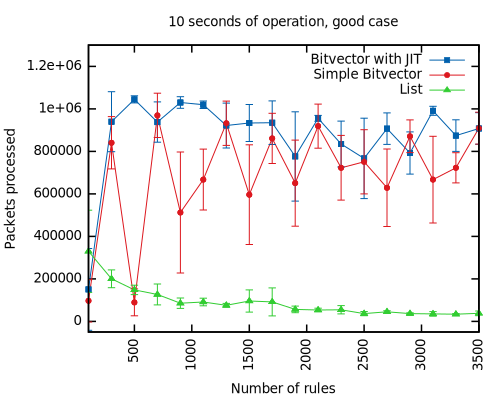
\includegraphics[width=\textwidth]{images/eval_b}
        \caption{Good case.}
        \label{fig:eval_good_case}
    \end{subfigure}
    ~
    \begin{subfigure}{.45\linewidth}
        \centering
        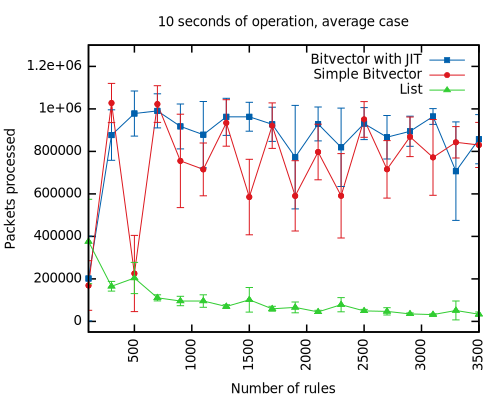
\includegraphics[width=\textwidth]{images/eval_a}
        \caption{Average case.}
        \label{fig:eval_average_case}
    \end{subfigure}
    ~
    \begin{subfigure}{.45\linewidth}
        \centering
        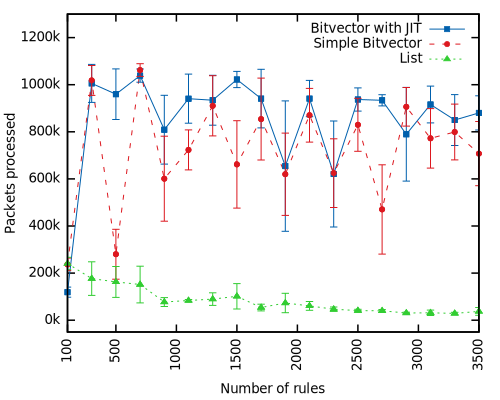
\includegraphics[width=\textwidth]{images/eval_w}
        \caption{Bad case.}
        \label{fig:eval_bad_case}
    \end{subfigure}
    \caption{Matching performance with 10 seconds of operation.}
\end{figure}

\begin{figure}
    \centering
    \begin{subfigure}{.45\linewidth}
        \centering
        \includegraphics[width=\textwidth]{images/eval_b_relative}
        \caption{Good case.}
        \label{fig:eval_good_case_relative}
    \end{subfigure}
    ~
    \begin{subfigure}{.45\linewidth}
        \centering
        \includegraphics[width=\textwidth]{images/eval_a_relative}
        \caption{Average case.}
        \label{fig:eval_average_case_relative}
    \end{subfigure}
    ~
    \begin{subfigure}{.45\linewidth}
        \centering
        \includegraphics[width=\textwidth]{images/eval_w_relative}
        \caption{Bad case.}
        \label{fig:eval_bad_case_relative}
    \end{subfigure}
    \caption{Relative matching performance (measured against the List algorithm).}
\end{figure}

\subsubsection{Insertion Time}
\label{sec:eval-ins}
Figure~\ref{fig:eval-times} shows the significant loss in efficiency when inserting rules into the code generating algorithm.
The two graphs show the duration of an update with different sized rule sets in the 
JIT implementation and in the conventional bitvector approach.
Unfortunately, adding rules with the \textsf{dpctl} tool is relatively slow itself, so that measurements using this tool
are uncertain and adding overhead to the algorithms' insertion performance.
Therefore, this test was executed on the two newly implemented modules separately and in only one matching dimension.
In order to compensate for the decreased complexity of this approach compared to the twelve dimensional OpenFlow matching,
a greater number of rules was inserted into each matching engine.
Because of the requirement that the matching engine has to be operable 
immediately after every update operation, every insertion implies a complete regeneration of the JIT code.
That behaviour induces the massive additional update time seen in the measured data.
A reduction might be possible by waiting if the next update is immediately following
and, if true, waiting for the JIT regeneration until no more updates arrive for a certain time.
The downside of this approach is the incorrect state of the JIT until it is rebuilt.

\begin{figure}
\centering
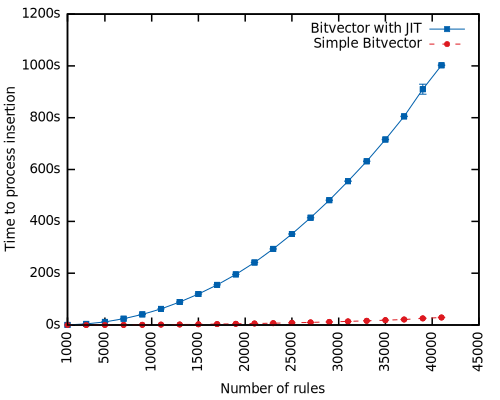
\includegraphics[width=0.6\textwidth]{images/eval_time}
\caption{Time needed to insert rules into the switch.}
\label{fig:eval-times}
\end{figure}

\subsubsection{Implementation Complexity}
The three algorithms are implemented in C.
To give a rough estimation of complexity, Table~\ref{table:loc} shows the 
approximate size of the implementation sizes measured in lines of code.
In comparison, the JIT implementation is smaller than the classic bitvector algorithm when performing a lookup.
However, the added complexity of the code generation is clearly visible.
The list is very small in inserting the entries.
When looking packets up, the list implementation is relatively large.
This is partly due to a relatively generic matching structure that is very 
easy to expand to more than the original twelve matching fields.

\begin{table}
  \centering
  \begin{tabularx}{\textwidth}{l|XXX}
  &List&Simple Bitvector&JIT Bitvector\\
  \hline
  Insertion&30&140&310\\
  Lookup&100&100&70\\
  \end{tabularx}
  \caption{Lines of code for all three implementations.}
  \label{table:loc}
\end{table}

\subsubsection{Memory Usage}

\begin{figure}[H]
\centering
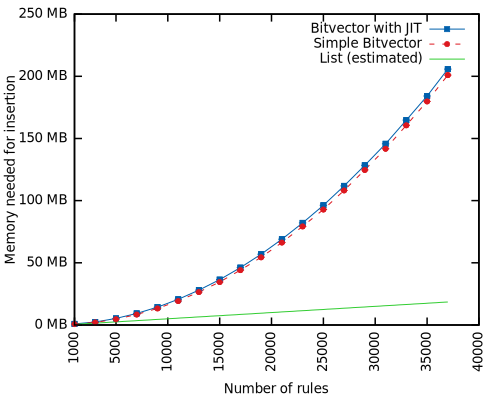
\includegraphics[width=0.6\textwidth]{images/eval_mem}
\caption{Memory needed to store rules in the switch. List memory is estimated.}
\label{fig:eval-mem}
\end{figure}

An increased memory consumption is the trade-off for using the bitvector implementation
instead of the list based lookup.
Figure~\ref{fig:eval-mem} shows a crude estimate of the difference.
Note that the data for the two bitvector implementations was obtained by measuring memory consumption of the separate implementation
similar to Section~\ref{sec:eval-ins}.
The memory consumption of the list implementation bases on source code analysis of 
the data structures generated by the list functions.
Even though this method implies an uncertainty, it is sufficient to recognize the difference in magnitudes.
The small overhead of the JIT implementation in comparison with the simple bitvector approach
arises from the size of the actual JIT compiled function.

\section{Conclusion}
Speeding up the matching process in the OpenFlow reference implementation switch has been accomplished successfully.
The bitvector algorithm itself achieves an impressive gain in classification 
performance in comparison to the linear lookup.
Further optimization resulted in the development of a just-in-time compiler 
that generates a special function for looking up values in a defined rule set.
Evaluation results show another increase of lookup performance for the JIT optimized algorithm.
However, the insertion time grows drastically for larger rule sets because 
of the time needed to regenerate the JIT compiled function for each new rule.

The evaluation also proves that the prize to pay for faster classification 
is an increasing usage of memory compared to the list implementation.
However, the JIT solution is in the same magnitude of memory consumption 
compared to the simple bitvector implementation. 
Another new benefit is the possibility to perform parallel lookups for each header dimension.
Only the bitvector aggregation step has to take place on one single node.

\section{Future Work}
Future work in this particular area can steer in manifold directions.
One of the main objectives is further optimization of the matching algorithm.
One possibility to speed up the switch is to reduce the time used for the JIT code generation.
Modifying the existing JIT function instead of deleting the old one and building 
a new one from scratch might be a worthwhile task.
This should save time when updating the rule set.
Especially in environments with fast-changing rule sets that idea may offer 
a significant advantage over the current implementation.

Another idea that comes to mind is to implement a heuristic which detects 
the most popular flows of the last time span in an operating switch.
After gathering traffic data for a while it might prove beneficial to tune 
the JIT function in such a way that the search for packet header data in a popular flow returns faster.
Also, the chronology of the stored bitvectors can be optimized in certain boundaries:
the order of bitvectors that do not overlap with each other is indifferent.
If often used bitvectors are placed closer to the front, the matching process 
can be sped up because it scans the result bitvector from left to right for the first set bit.
However, if bitvectors overlap, their relative order must remain.
Depending on the type of traffic, these optimizations may either cause a massive performance boost or no real advantage.
The latter case enters if there are no real flows recognizable in the traffic because it is very sparse.
Nevertheless, in most real world cases there exist observable traffic patterns~\cite{elephantmice}.

\appendix
\section{Appendix}
\pagestyle{empty}
\thispagestyle{scrheadings}
\begin{algorithm}
\begin{multicols}{2}
\lstinputlisting[
    language={[x86masm]Assembler},
    breaklines=true,
    numbers=left,
    texcl=true,
    xleftmargin=5.0ex,
    basicstyle=\footnotesize\ttfamily,
    keywordstyle=\bfseries\color{red},
    commentstyle=\itshape\color{grey},
    identifierstyle=\color{blue},
    %deletekeywords{movl},
    morekeywords={retq,cmpq},
    numberstyle=\tiny
    ]
    {jit_listing.asm}
\end{multicols}
\captionof{lstlisting}{Assembly code generated by the JIT compiler.}
\label{lst:jit}
\end{algorithm}

\newpage
\addcontentsline{toc}{section}{References}
\interlinepenalty=10000
\bibliographystyle{acm}
\bibliography{references,paper-build/conferences-crossref,rfc}

\end{document}
